\subsection{\SubsecOnlineNesting} \label{subsec:nest_online}
%----------------------------------------------------------

オンライン・ネスティング実験を実行する際には、以下の2つの制約が存在する。
\begin{itemize}
\item 子領域の積分時間は、親領域の積分時間と一致していなければならない。
\item 親領域の時間ステップは、子領域の時間ステップの倍数でなければならない。
\end{itemize}
一方で、親領域と子領域で鉛直層数、鉛直レベル、地図投影法、物理スキームが一致している必要はない。
オンライン・ネスティング実験では、全ての領域の計算は同時に実行される。
現在のバージョンでは、\scalerm は一方向ネスティングのみ対応する。
ネスティングの段数は最大で10段まで可能である。

\scalerm のオンライン・ネスティング実験では、複数領域の時間積分を逐次的でなく並列的に行う。
図\ref{fig_mpisplit}に示すように、MPIプロセスはいくつかのグループに分割される。
各々のグループは一つの領域を担当し、独立したモデルのように計算を進める。
複数の領域を立ち上げるために、\verb|launch.conf|という設定ファイルが実行時に必要である。

\begin{figure}[ht]
\begin{center}
  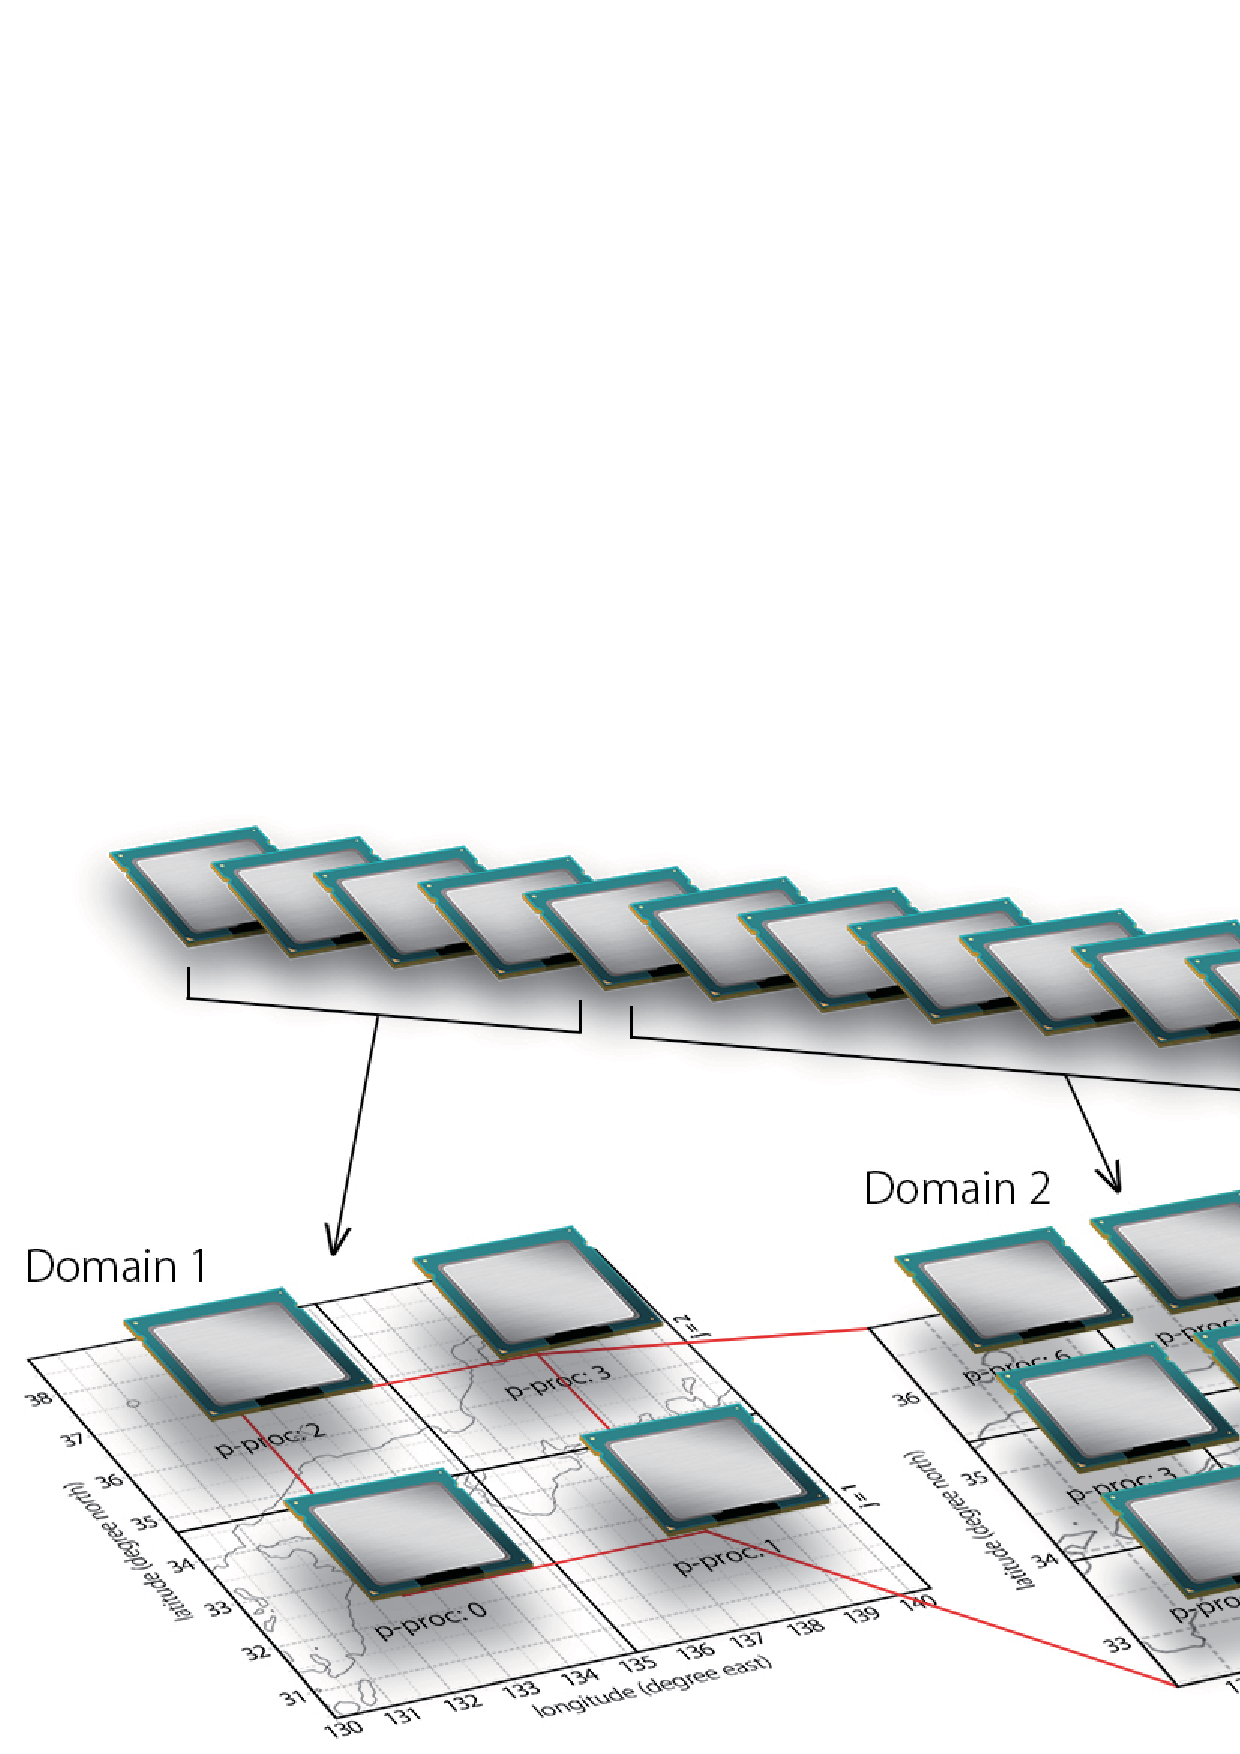
\includegraphics[width=0.8\hsize]{./figure/mpisplit_nesting.pdf}\\
  \caption{ オンライン・ネスティング実験におけるMPIプロセスの配分。
           この例では 13 のプロセスが最初に立ち上げられ、これらを適切に分配する。
           つまり、Domain 1では$2 \times 2$の4-MPI並列計算、
           Domain 2では$3 \times 3$の9-MPI並列計算が行われる。
           MPI通信によってDomain 1からDomain 2へデータを受け渡しながら時間積分が進められる。}
  \label{fig_mpisplit}
\end{center}
\end{figure}


以下では、最も単純なオンライン・ネスティングの例として2段ネスティングを説明する。
%
ここで記述される実験セット一式は、サンプルファイル
\verb|${Tutorial_dir}/real/sample/USER.online-nesting.sh|を
USER.shに名前を変更して、「\makeconftool」を実行することで作成される
(第\ref{sec:basic_makeconf}節を参照)。
以下の説明では、各領域に対する地形/土地利用データと初期値/境界値データの作成を終えているとする。
地形データの作成手順は、第\ref{subsec:nest_topo}節に示した通りである。

\subsubsection{オンライン・ネスティングの設定}
親領域と子領域のそれぞれの設定ファイル(\verb|run.***.conf|)において、
オンライン・ネスティングのための設定を以下のように\namelist{PARAM_NEST}に追加する。

\noindent {\gt \verb|run.d01.conf|の設定}\\
\editboxtwo{
\verb|&PARAM_NEST|                          & \\
\verb| ONLINE_DOMAIN_NUM        = 1,      | & 領域の番号。外側から1番。\\
\verb| ONLINE_IAM_PARENT        = .true., | & \\
\verb| ONLINE_IAM_DAUGHTER      = .false.,| & \\
\verb| ONLINE_BOUNDARY_USE_QHYD = .true., | & \\
\verb| ONLINE_AGGRESSIVE_COMM   = .true., | & \\
\verb|/| \\
}
~\\
\noindent {\gt \verb|run.d02.conf|の設定}\\
\editboxtwo{
\verb|&PARAM_NEST| & \\
\verb| ONLINE_DOMAIN_NUM        = 2,      | & 領域の番号。外側から1番。\\
\verb| ONLINE_IAM_PARENT        = .false.,| & \\
\verb| ONLINE_IAM_DAUGHTER      = .true., | & \\
\verb| ONLINE_BOUNDARY_USE_QHYD = .true., | & \\
\verb| ONLINE_AGGRESSIVE_COMM   = .true., | & \\
\verb|/| \\
}

\nmitem{ONLINE_DOMAIN_NUM}は、
領域のID番号であり、外側領域から内側領域へ順番に番号を振っていく。
上の例において、親領域と子領域のID番号はそれぞれ1番と2番である。\\
\nmitem{ONLINE_IAM_PARENT}と\nmitem{ONLINE_IAM_DAUGHTER}は、
各領域がその親領域や子領域を持っているかを指定する項目である。
$N$番目の領域において\nmitem{ONLINE_IAM_PARENT} が \verb|.true.|であれば、
$N$番目の領域の計算データは$N+1$の領域番号をもった子領域に送られる。
\nmitem{ONLINE_IAM_DAUGHTER} が \verb|.true.|であれば、
$N$番目の境界データは$N-1$番の領域番号をもった親から受け取る。
最も外側の領域は親領域としてのみ働き、最も内側の領域は子領域としてのみ働く。
一方で、中間的な領域は親領域と子領域の両方を担うので、
\nmitem{ONLINE_IAM_PARENT}と\nmitem{ONLINE_IAM_DAUGHTER}は共に\verb|.true.|である。
表\ref{tab:triple_nested}は$N$段ネスティング実験の設定を示している。

\begin{table}[htb]
\begin{center}
\caption{N段ネスティングの設定例}
\begin{tabularx}{150mm}{|l|l|l|X|} \hline
 \rowcolor[gray]{0.9} 領域 & \verb|ONLINE_DOMAIN_NUM| & \verb|ONLINE_IAM_PARENT| & \verb|ONLINE_IAM_CHILD|\\ \hline
 最外領域 & 1               & .true.  & .false. \\ \hline
 中間領域 & 2\verb|〜|(N-1) & .true.  & .true. \\ \hline
 最内領域 & N               & .false. & .true. \\ \hline
\end{tabularx}
\label{tab:triple_nested}
\end{center}
\end{table}

\nmitem{ONLINE_BOUNDARY_USE_QHYD}は、境界条件として凝結物の値を使うかを指定する。
外部入力データから側面境界条件を作成するときには、凝結物の値は通常使われない。
しかし、ネスティング実験では、二領域間で物理スキームが違わないために、
親領域で計算された凝結物を子領域の境界条件として与えることができる。
計算領域の内部に影響を与えるような、流入境界付近での雲や降水の発生の遅れが、
この改善策によって抑制されると考えられる。


\subsubsection{ランチャーの設定}
\label{subsubsec:launch}
オンライン・ネスティング実験には、
\verb|run.***.conf|の他に、起動用設定ファイル\verb|launch.conf|が必要である。
\editboxtwo{
\verb|&PARAM_LAUNCHER|      & \\
\verb| NUM_DOMAIN  = 2,|    & 領域の数\\
\verb| PRC_DOMAINS = 4, 16,| & それぞれの領域で使用するMPIプロセス数 (領域の数だけ必要)\\
\verb| CONF_FILES  = run.d01.conf, run.d02.conf,| & それぞれの領域の設定ファイル (領域の数だけ必要)\\
\verb|/|& \\
}
\nmitem{PRC_DOMAINS}と\nmitem{CONF_FILES}の記載順は対応している必要がある。
上記の例の場合は、親領域は4-MPI並列、子領域は16-MPI並列で実行するように指定されている。
\verb|launch.conf|で指定するMPIプロセス数は、各々の領域の設定ファイル (\verb|run.***.conf|)
で指定された総MPIプロセス数(\verb|PRC_NUM_X|$\times$\verb|PRC_NUM_Y|)と一致させなければならない。

実行時には、シングル領域計算の場合とは異なり、計算全体で使用するMPIプロセス数を指定する。
例えば、上記の場合だと20プロセスを指定する。
\begin{verbatim}
 $ mpirun  -n  [プロセス数]  ./scale-rm  launch.conf
\end{verbatim}

複数領域の計算が同時に実行されるときに、混同を避けるために、
異なるファイル名を入出力ファイルに対して使用しなければならない。
例えば、「\makeconftool」によって用意した設定ファイルでは、
ヒストリ出力のファイル名を\verb|history_d01.pe***.nc, history_d02.pe***.nc|としている。

実行時に次のようなメッセージが出力されて、計算が異常終了することがある。
これは、子領域の計算領域が親領域の計算領域よりも大きいことを意味するエラーメッセージである。
このようなメッセージが出た場合は、地形・土地利用データ、および初期値/境界値の作成から
やり直し、設定が適切であるか再度確認されたい。
\msgbox{
  \verb|ERROR [COMM_CARTESC_NEST_domain_relate] region of daughter domain is larger than that |\\
  \verb| of parent| \\
}

\subsubsection{MPIプロセスの分配に関するガイドライン}
%-------------------------------------------------------------------------
オンライン・ネスティング実験では、図\ref{fig_mpisplit}に示したように、
複数の領域間でMPIプロセスを共有しない。
つまり、それぞれのMPIプロセスは特定の領域の一部分を担当することになる。
このため、ユーザはいくつのMPIプロセスを各領域に割り当てるかを決める必要がある。
この割り当て配分が適切でない場合は、長い待ち時間が発生する。
これを避けるためには、各プロセスにおける時間積分の計算量がプロセス間で可能な限り揃うように、
MPIプロセスを配置するのが合理的である\footnote{正確を期すなら演算量を見積もる必要がある。}。
ここで、時間積分の計算量は、格子数とタイムステップ数の積として定義する。

ここでは、N段ネスティングを考える。
n番目の領域の{\XDIR}、{\YDIR}、{\ZDIR}の格子数をそれぞれ\verb|IMAX_n|、\verb|JMAX_n|、\verb|KMAX_n|と表す。
また、n番目の領域の時間ステップ\nmitem{TIME_DT}を\verb|DT_n|と表す。
この時、一番外側の領域(n=1)の時間積分のタイムステップ\verb|DT_1|を基準とし、この時間を積分するのに必要なn番目の領域の計算ステップ数は、
\begin{eqnarray}
 \verb|TSTEP_n| = \verb|DT_1| / \verb|DT_n|  \nonumber
\end{eqnarray}
と表される。領域全体での計算量は、領域が持つ格子数を掛けて
\begin{eqnarray}
 \verb|OPR_n| = \verb|IMAX_n| \times \verb|JMAX_n| \times \verb|KMAX_n| \times \verb|TSTEP_n| \nonumber
\end{eqnarray}
と見積もられる。
したがって、n番目の領域に配分するMPIプロセス数の目安は、
\begin{eqnarray}
 \verb|MPI_total| \times \frac{ \texttt{OPR\_n} }{ \sum_{m=1}^N \texttt{OPR\_m} }
\end{eqnarray}
と見積もられる。
ここで、\verb|MPI_total|は全MPIプロセス数である。


{\XDIR} と{\YDIR}に分配するプロセス数\nmitem{PRC_NUM_X, PRC_NUM_Y}には任意性が残る。
\verb|IMAX|と\verb|JMAX|の違いができるだけ小さくなるように、これらを設定することが推奨される。
その理由は、このような設定によってハロ領域を減らせるためである。
結果的に、計算機の演算性能を引き出しやすいと考えられる
\footnote{ただし、「京」のようにスレッド並列も併用するハイブリッド並列の場合には、
スレッド間の演算量の不釣り合いを小さくするために{\XDIR}よりも{\YDIR}の格子点数を大きく取る必要がある。}。


上記の説明では、格子点数と積分時間の時間刻み幅のみを考慮した。
しかし、現実大気のネスティング実験のような実計算では、各物理過程の時間間隔の違いや、
領域内や領域間のMPI通信にかかる時間の違いも計算時間に影響を及ぼす。
オンライン・ネスティングの設定では、通常は最内領域で最も計算負荷が高く、
そこでのMPI通信の待ち時間が最小となるようにプロセスを分配するのが効率的であることが多い。
大規模計算、 長期積分、アンサンブル実験を行う場合は、
上記の方法で効率的な配分を大まかに見積もり、微調整することを勧める。
